\subsection{Постановка задачи на разработку программы}
\tab[0.75cm]Программа должна соответствовать требованиям, представленным в
Техническом
Задании.

\bigskip
\subsubsection{Задачи работы (Андроид-клиент)}
\smallskip
\begin{my_enumerate}
\item Реализовать возможность просмотра списка доступных магазинов с акционными товарами
\item Реализовать представление текущих акций для конкретного магазина:
    \begin{my_enumerate}
    \item В виде общего списка
    \item По категориям
    \end{my_enumerate}
\item Реализовать постепенную загрузку товаров магазинов (по страницам) для экономии трафика и меньшей нагрузкой на мобильное устройство
\item Реализовать регистрацию через мобильное приложение
\item Реализовать вход в аккаунт через мобильное приложение
\item Реализовать возможность смены аккаунта
\item Реализовать возможность создания списков покупок c разными названиями
\item Реализовать возможность удаления списка покупок
\item Реализовать возможность добавления товара в список покупок
\item Реализовать возможность удаления товара из списка покупок
\item Реализовать возможность добавления в список покупок пользовательских товаров, котороых нет в магазине (см. терминологию)
\item Реализовать возможность просмотра подобранных программой товаров согласно запросу пользователя
\item Реализовать добавление подобранных товаров в список покупок
\item Реализовать предварительное отображение элементов каждого списка покупок до их открытия
\item Реализовать отображение всплывающих подсказок при долгом нажатии на элементы управления button (кнопка)
\item Реализовать перенаправление в настройки сети для последующего включения интернета при отсутствии интернет-соединения
\item Реализовать отображение индикатора процесса загрузки данных с сервера
\item Реализовать обучающий фрагмент в разделе help (см. терминологию), содержащий руководство пользователя по управлению программой
\end{my_enumerate}

\subsubsection{Задачи работы (серверная часть)}

\smallskip
\begin{my_enumerate}
    \item Реализовать crawling веб-страниц для сбора актуальной информации об акционных товарах
        \begin{my_enumerate}
            \item Реализовать spider для каждого магазина для сбора данных с их веб-страниц
            \item Реализовать модуль text\_processor для очистки собранных текстовых данных
            \item Реализовать ``модульные'' xpath селекторы, для оперативного восстановления при изменении дизайна сайта
        \end{my_enumerate}
    \item Модуль pipelines: реализовать добавление товаров в базу данных посредством отправки запросов REST API (REST API и база данных реализованы напарником)
    \item Модуль pipelines: реализовать запись акционных товаров со всех магахинах в JSON файл
    \item Реализовать email уведомления администраторам сервиса об ошибках и неполадках в работе сервера
    \item Реализовать ежедневное обновление акций для поддержания актуальности
\end{my_enumerate}


\subsection{Описание алгоритма и функционирования программы}

\subsubsection{Описание построения Андроид приложения}
В андроид приложении задумано 4 активности (см. терминологию) и 2 фрагмента (см. терменологию)\\
\begin{my_enumerate}
    \item \textbf{LoginActivity} Рис \ref{login_activity}. Активность,
        формирующая интерфейс входа пользователя в систему. Является самой
        первой ативностью, которая загружается всегда при запуске приложения,
        но если пользователь до этого момента уже входил в свой аккаунт, его
        данные сохранены в shared preferences (см. терминологию) и эта
        активность опускается. В этой активности 2 поля для ввода текста
        (логина и пароля) и 3 кнопки (войти, зарегистрироваться и продолжить
        использование без входа в аккаунт);
    \item \textbf{RegisterActivity} Рис \ref{register_activity}.  Активность
        для регистрации пользователя.  Имеет 2 поля для ввода текста (логинa и
        пароля), и 2 кнопки: ``Зарегистрироваться'' (для новых пользователей) и
        ``Войти'' (для пользователей, уже имеющих аккаунт). Пользователь также
        может вернуться в активность для входа в систему посредством нажатия
        систесной кнопки ``назад'';
        \begin{figure}[h!]
            \centering
            \minipage{0.45\textwidth}
            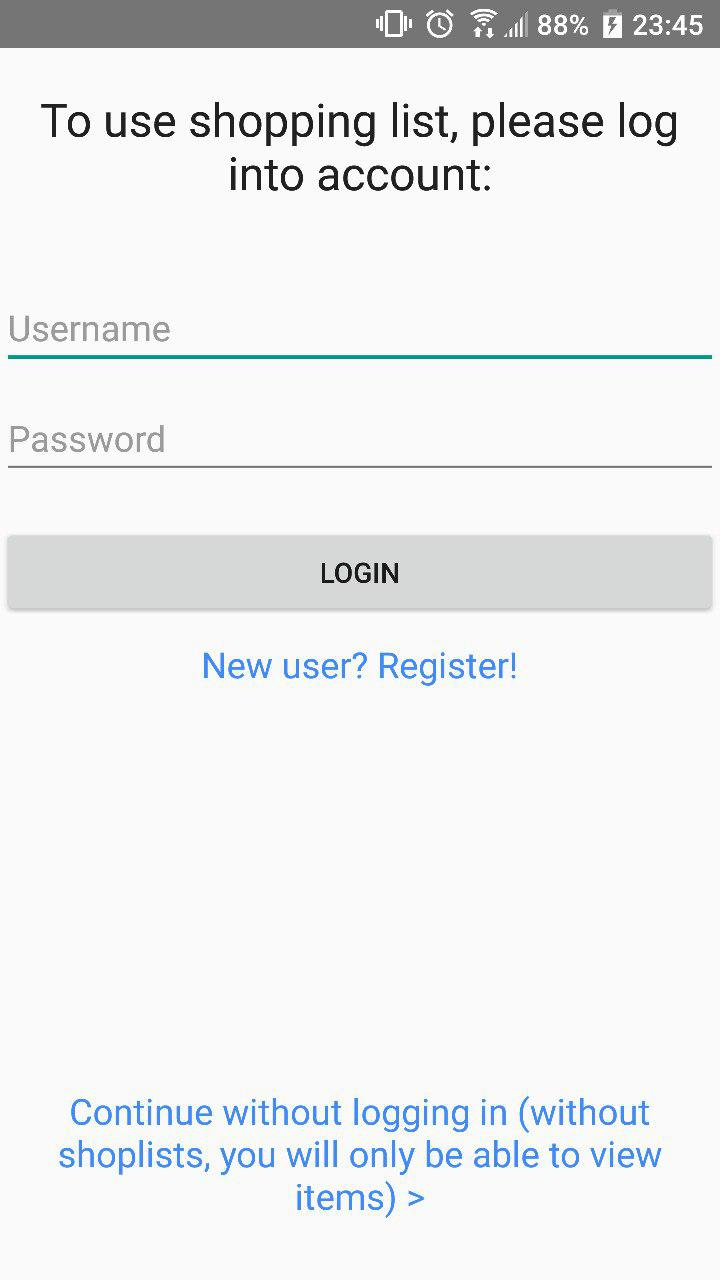
\includegraphics[height=0.42\textheight]{./screenshots/3/login.jpg}
            \caption{\small{Активность для входа в аккаунт пользователя}}
            \label{login_activity}
            \endminipage\hfill
            \minipage{0.45\textwidth}
            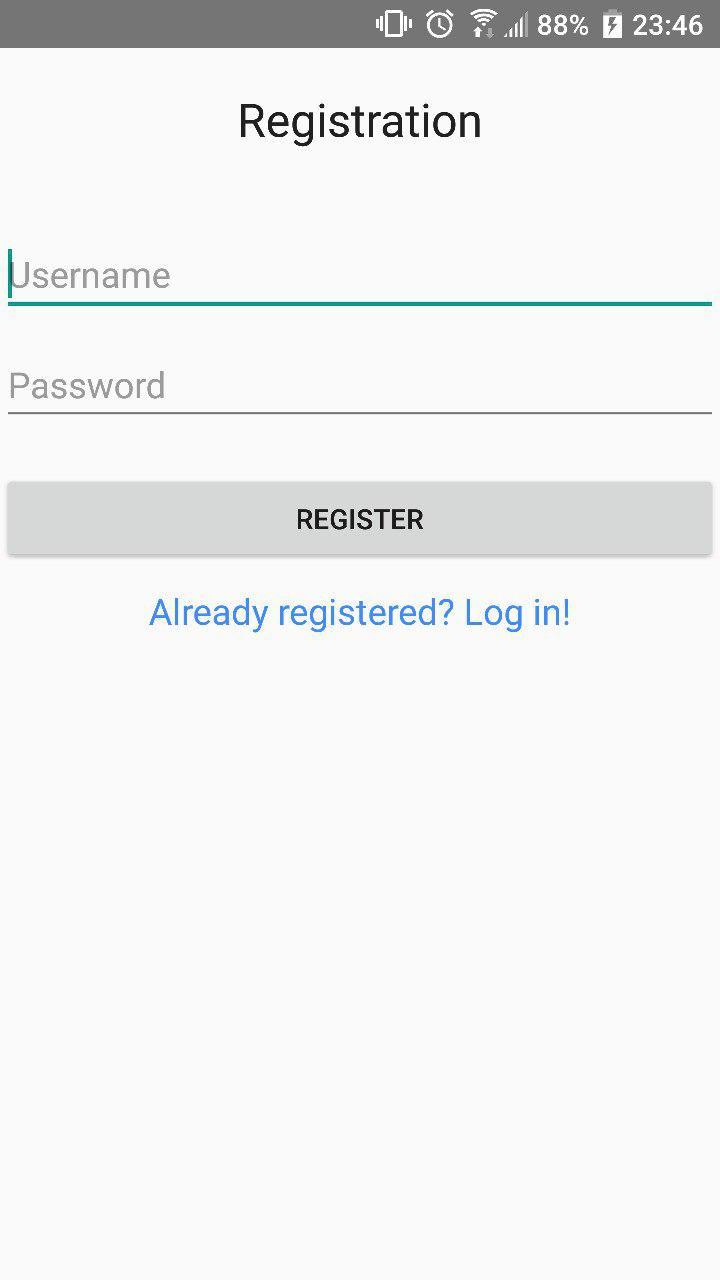
\includegraphics[height=0.42\textheight]{./screenshots/3/register.jpg}
            \caption{\small{Активность для регистрации аккаунта пользователя}}
            \label{register_activity}
            \endminipage
        \end{figure}
    \item \textbf{MainActivity} Главная активность, содержащая 2 дочерних
        фрагмента, toolbar и BottomNavigationView (см. терминологию).\\
        Фрагменты:
        \begin{my_enumerate}
            \item \textbf{HomeFragment} Рис \ref{home_fragment}. Фрагмент, содержащий список всех
                товаров. Список может быть отфильтрован по магазинам и по
                категориям. Содержит toolbar, в котором есть выпадающий список
                для выбора магазина, кнопка для выхода/входа из/в аккаунт(а), и
                меню опций;
            \item \textbf{ShopListsPreviewFragment} Рис \ref{shoplist_fragment}. Фрагмент, содержащий список
                всех списков покупок. Списки покупок упорядочены в виде
                карточек с предпросмотром в них добавленных товаров магазина и
                пользовательских товаров. Нажатие по одному из них открывает
                активность ShopListActivity, содержащюю подробную информацию об
                элементах списка покупок. Долгое нажатие по одному из списков
                вызовет диалоговое окно, в котором спросится подтверждение
                намерения удалить данный список покупок. В элементе toolbar в
                этом фрагменте есть кнопка для входа/выхода в/из аккаунт(а), и
                кнопка для добавления нового списка покупок. Использование
                фрагмента не доступно неавторизованным пользователям;
        \end{my_enumerate}
        \begin{figure}[h!]
            \centering
            \minipage{0.45\textwidth}
            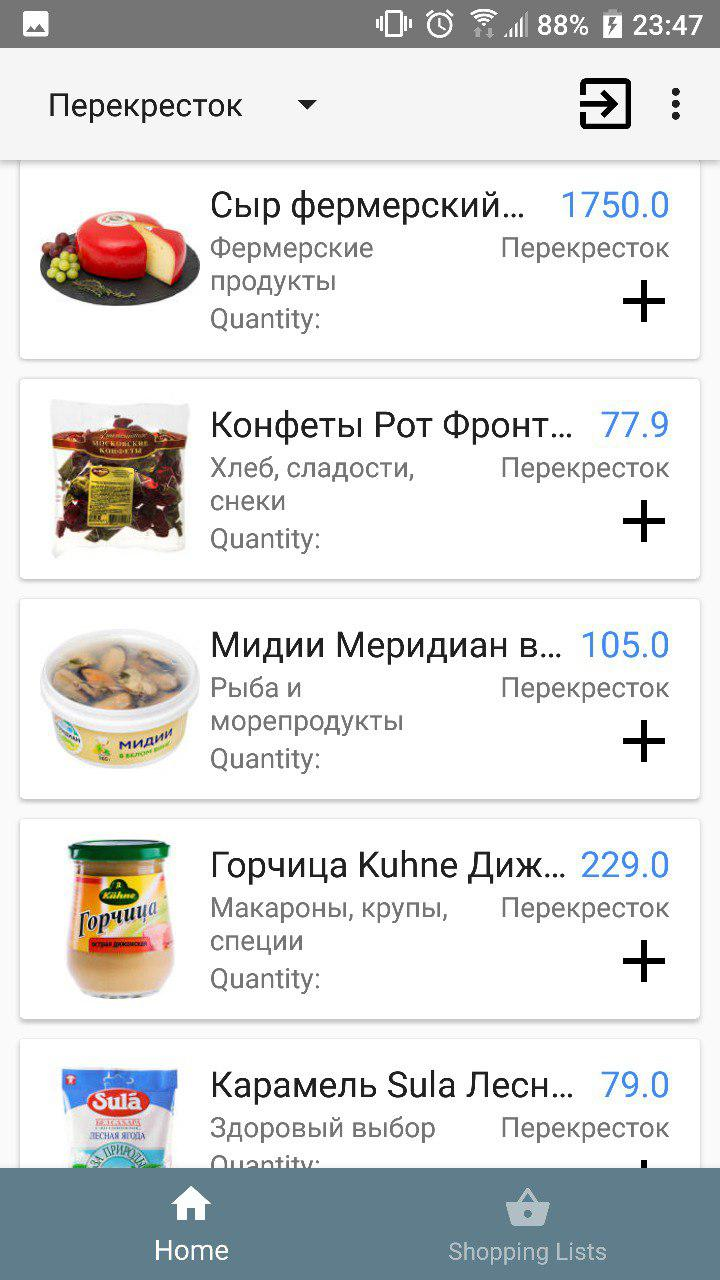
\includegraphics[height=0.42\textheight]{./screenshots/3/home.jpg}
            \caption{\small{MainActivity. Фрагмент со списком товаров магазинов}}
            \label{home_fragment}
            \endminipage\hfill
            \minipage{0.45\textwidth}
            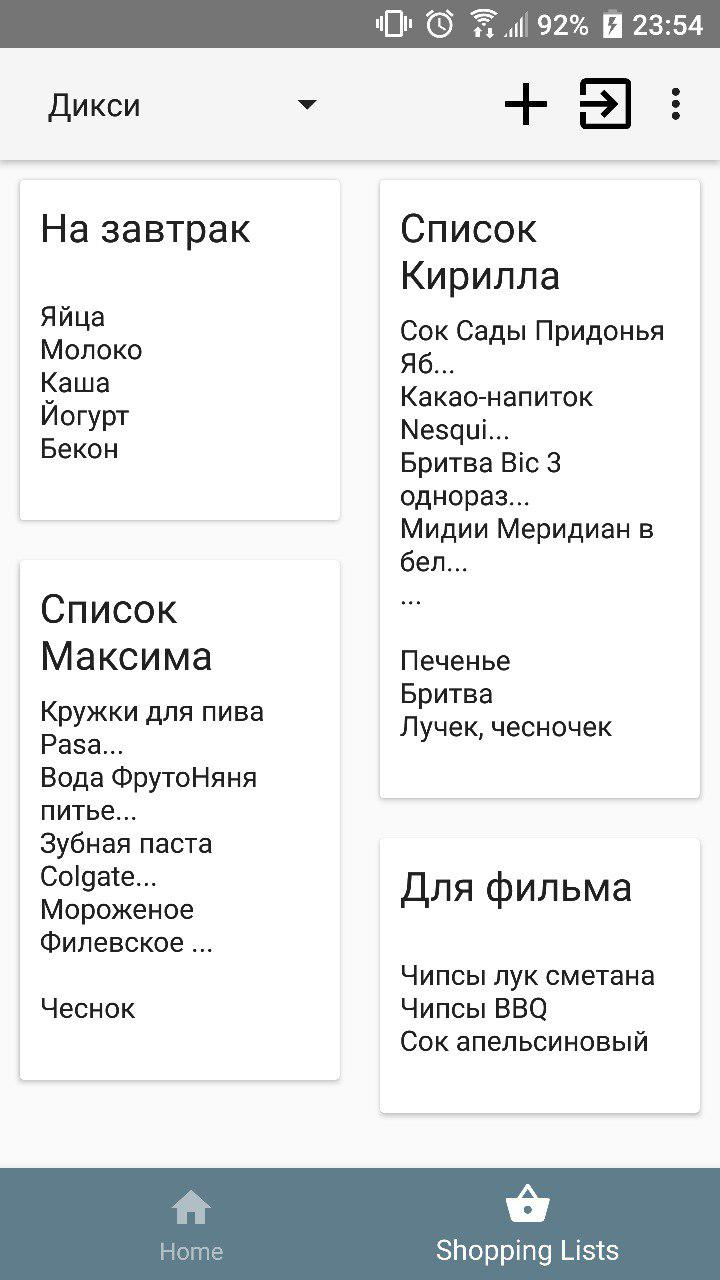
\includegraphics[height=0.42\textheight]{./screenshots/3/all_shoplists.jpg}
            \caption{\small{MainActivity. Фрагмент со всеми списками покупок}}
            \label{shoplist_fragment}
            \endminipage
        \end{figure}
    \item \textbf{ShopListActivity} Рис \ref{shoplist1}, рис \ref{shoplist2}. Активность, содержащая подробную информацию
        о конкретном списке покупок. В элементе toolbar отображается кнопка
        ``назад'', название списка покупок, и итоговая сумма по всем товарам, в
        стандартной для товаров валюте. В центре активности расположен список
        товаров магазина, а под ним - список пользовательских товаров. В свою
        очередь, каждый пользовательский товар содержит список подобранных
        товаров под данный из магазинов. Использование активности не доступно
        неавторизованным пользователям
\begin{figure}[h!]
    \centering
    \minipage{0.45\textwidth}
    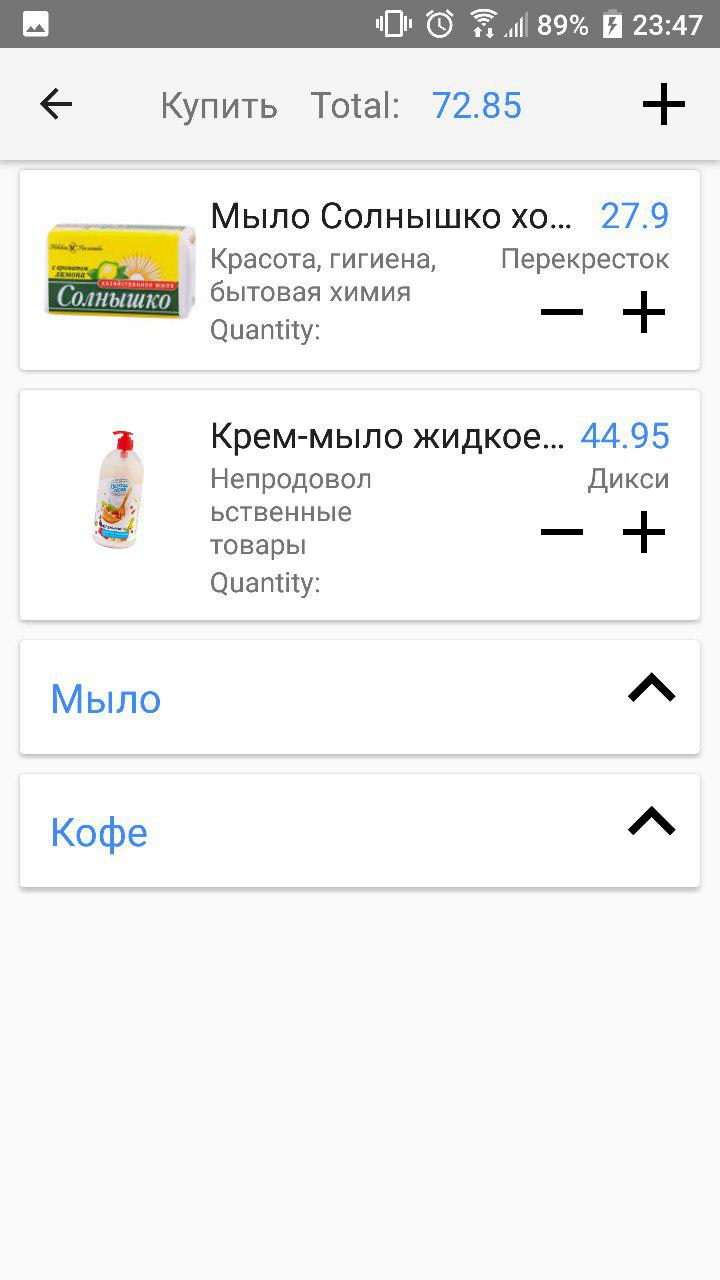
\includegraphics[height=0.42\textheight]{./screenshots/3/shoplist.jpg}
    \caption{\small{ShopListActivity}}
    \label{shoplist1}
    \endminipage\hfill
    \minipage{0.45\textwidth}
    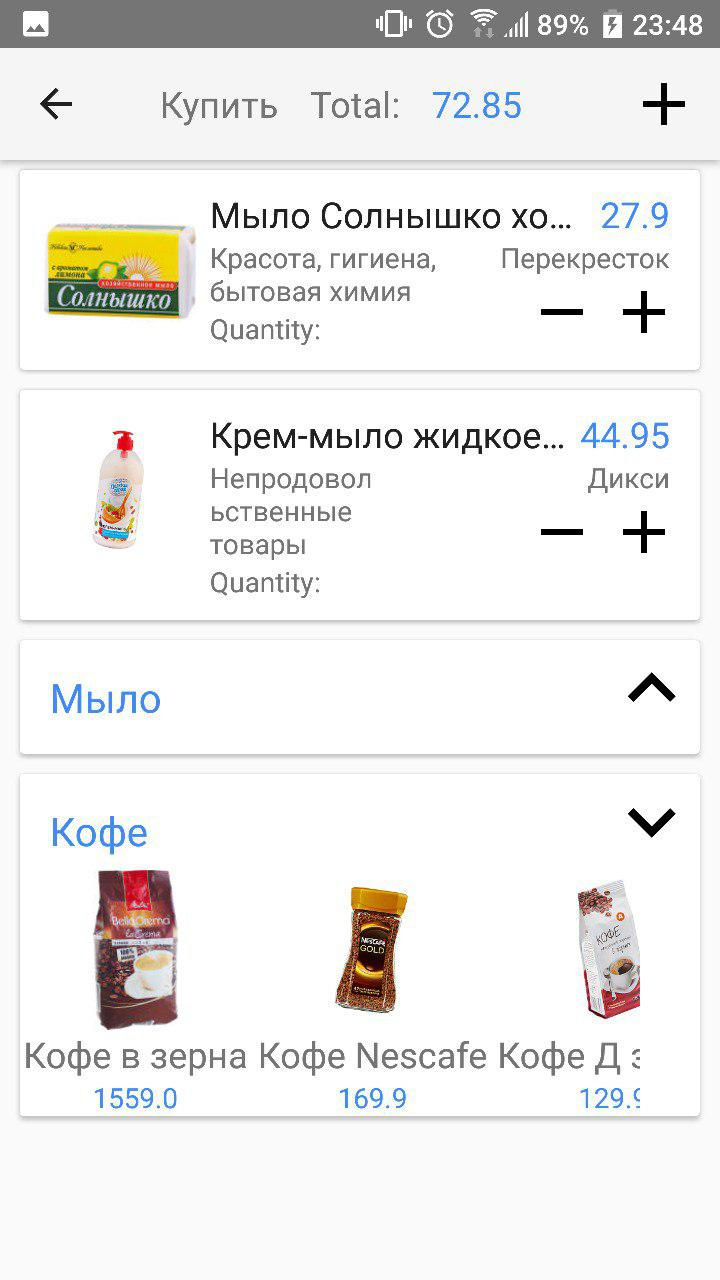
\includegraphics[height=0.42\textheight]{./screenshots/3/shoplist_custom_fold.jpg}
    \caption{\small{ShopListActivity. Показаны соотретствующие пользовательскому товару товары их магазинов}}
    \label{shoplist2}
    \endminipage
\end{figure}
\end{my_enumerate}

\subsubsection{Описание построения crawler'a}

В crawler'e веб-страниц магазинов предусмотрены следующие модули:
spiders/dixy\_spider, spiders/perekrestok\_spider, text\_processor,
dixy\_selectors, perekrestok\_selectors, settings, config, notify и pipelines.\\
\begin{my_enumerate}
    \item \textbf{dixy\_spider} описывает класс DixySpider, унаследованный от
        Scrapy.Spider. Отвечает за получение исходного кода страницы магазина
        ``Дикси'', его парсинга при помощи ``модульных'' xpath селекторов (см.
        терминологию), перехода по страницам на сайте. Формирует объекты классы
        DixyItem и передаёт далее модулю pipelines на обработку;
    \item \textbf{perekrestok\_spider} описывает класс PerekrestokSpider,
        функционал идентичен DixySpider, но действует на сайте магазина
        ``Перекресток'';
    \item \textbf{text\_processor} содержит функции обработки текста при помощи
        регулярных выражений и базовых операций со строками;
    \item \textbf{dixy/perekrestok selectors} содержат соответствующие xpath
        селекторы для веб-страниц магазинов. Выделение этой логики в отдельный
        модуль - корневая причина модульности приложения. В случае изменения
        дизайна сайта, кроулинг которого происходит, админимтратору придётся
        изменить лишь одну строчку для одного элемента на странице;
    \item \textbf{settings, config} содержат настройки и конфигурацию кроулера;
    \item \textbf{pipelines} содержит методы для обработки объектов DixyItem и
        PerekrestokItem. Модуль так же совершает POST запрос на сервер
        приложения для добавления товара в базу данных, и сохраняет все объекты
        в JSON файл
\end{my_enumerate}

\subsection{Ежедневное обновление акций}
Процесс ежедневного обновления акций необходимо проводить, чтобы акции в приложении всегда были актуальными.

На сервере запущена cron job (см. терминологию), котрая каждый день в 2:00 ночи в 6:00 утра запускает процесс кроулинга акций во всех магазинах:

\begin{small}
    \begin{verbatim}
         00 2,6 * * * cd /home/hes/Projects/crawler/easysales && ./crawl_all.sh > /home/hes/crawler.log 2>&1
    \end{verbatim}
\end{small}

Скрипт crawl\_all.sh отвечает за поочередный запуск всех spider'ов. Далее, по
цепочке, спайдеры собирают данные с сайтов при помощи xpath селекторов,
используют модуль text\_processor для очистки собранных данных от non-breaking
space символов, длинных пробелов и других символов. Формируются <Shop>Items,
которые затем отправляются в модуль pipelines. Классы <Shop>Items, процесс
добавления Item'a в базу и модель с селекторами для магазина ``Перекресток''
описаны ниже.

Классы DixyItem и PerekrestokItem унаследованы от EasySalesItem, базового
товара приложения. Его поля всегда заполнены, то есть не могут иметь значения
null.

\begin{small}
    \begin{verbatim}
class EasySalesItem(scrapy.Item):
    name = scrapy.Field()
    newPrice = scrapy.Field()
    imageUrl = scrapy.Field()
    shopId = scrapy.Field()
    crawlDate = scrapy.Field()


class DixyItem(EasySalesItem):
    category = scrapy.Field()
    oldPrice = scrapy.Field()
    discount = scrapy.Field()
    dateIn = scrapy.Field()
    dateOut = scrapy.Field()
    condition = scrapy.Field()


class PerekrestokItem(EasySalesItem):
    category = scrapy.Field()
    oldPrice = scrapy.Field()
    \end{verbatim}
\end{small}

Отправка объекта класса Item в базу данных происходит при помощи API запроса на
сервер:


\begin{small}
    \begin{verbatim}
class DataBaseWriterPipeLine(object):

    def process_item(self, item, spider):
        requests.post(const['ADD_ITEM_API'],
                      data=json.dumps(dict(item)),
                      headers=const['REQUEST_HEADERS'])
        return item
    \end{verbatim}
\end{small}

Xpath селекторы для магазина ``Перекресток''. Модульность и простота использования написанного фрагмента кода достигается тем, что при изменении дизайна сайта магазина, возникает необходимость исправить всего несколько строчек в приведённом фрагменте. Таким образом, частично решается проблема всех кроулеров - поломка, в случае изменения дизайна сайта. А поскольку большинство кроулеров не используют такой модульный подход, времени и сил на починку уходит гораздо больше, так как приходится править множество файлов во многих местах.

\begin{small}
    \begin{verbatim}
# Start urls.
#
URLS = ['https://www.perekrestok.ru/catalog']
URL_CORE = 'https://perekrestok.ru'

# Categiries.
#
CATEGORIES = '//a[@class="xf-catalog-categories__link"]/@href'
CATEGORIES_TEXT = '//span[@class="xf-catalog-categories__text"]/text()'
POST_CATEGORY = '//span[@class="xf-breadcrumbs__current"]/text()'
CURRENT_CATEGORY = '//h1[@class="xf-caption__title"]/text()'

ROOT_NODE = '//ul[@id="catalogItems"]'
ITEM = 'li/div[contains(@class, "xf-product")]'

# Item attributes.
#
NAME = 'div[@class="xf-product__title xf-product-title"]/a[@class="xf-product-\
title__link js-product__title"]/text()'
IMG = 'figure/a/img/@data-src'
NEW_PRICE = 'div/div[contains(@class, "xf-product-cost__current")]/@data-cost'
OLD_PRICE = 'div/div[contains(@class, "xf-price xf-product-cost__prev")]/@data-cost'

# Pagination selector.
#
# next_page = '//li[@class="next"]/a/@href'
NEXT_PAGE = '//a[contains(@class, "xf-paginator__item js-paginator__next")]/@href'
    \end{verbatim}
\end{small}
